\documentclass[border=3mm]{standalone}
\usepackage{tikz}
\usetikzlibrary{angles}

\begin{document}

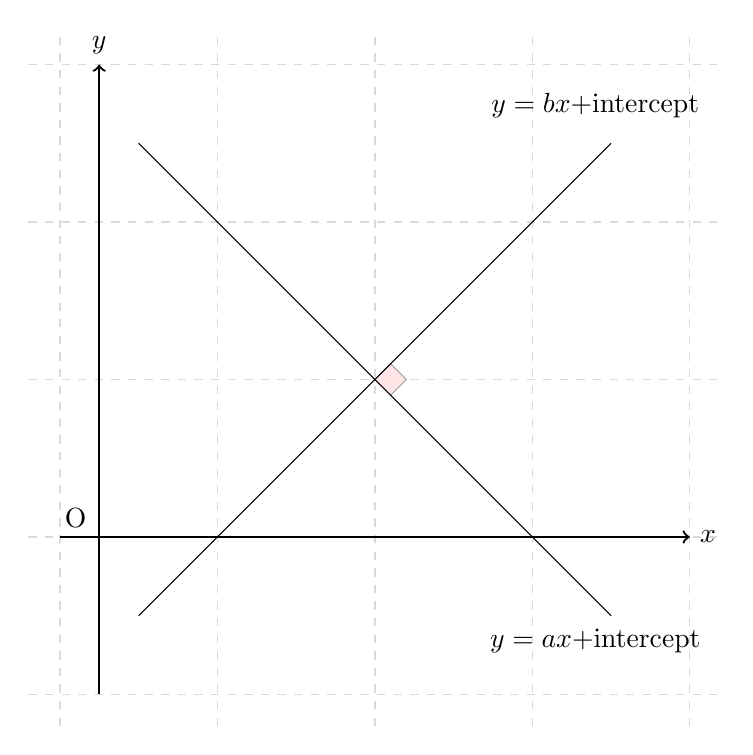
\begin{tikzpicture}[scale=2]
% define grid lines
\draw[help lines, color=gray!30, dashed, line width=0.5pt] (-2.2,-2.2) grid (2.2,2.2);

% mark right angles
\coordinate [label={O}] (O) at (-1.9,-1);
\filldraw[fill=red!10,draw=gray!70] (1/10,-1/10) -- (2/10, 0) -- (1/10,1/10) -- (0,0);

% label the lines
\coordinate [label={$y=ax+$intercept}] (O) at (1.4,-1.8);
\coordinate [label={$y=bx+$intercept}] (O) at (1.4,+1.6);

% define axis lines
\draw[->,thick] (-2,-1)--(2,-1) node[right]{$x$};
\draw[->,thick] (-1.75,-2)--(-1.75,2) node[above]{$y$};

% draw two orthogonal lines
\draw[black] (-1.5,-1.5) -- (1.5,1.5);
\draw[black] (1.5,-1.5) -- (-1.5,1.5);

\end{tikzpicture} 

\end{document}
